\chapter{心电信号的预处理及特征提取算法}
\section{心电信号的去噪算法}
\subsection{常用的去噪方法}
临床上实际获得心电图就是真正的心电信号与各类干扰噪声信号混叠而成的波形。因此,降低噪声对心电信号的影响一直是心电检测的一个重要问题\cite{11}。 

Thakor 研究了心电信号中各成分(包括噪声)的频谱特性分布\cite{12},如\autoref{fig:401}所示。由图可见心电各波段频谱有一定差异,其中 QRS 波群频率较高,
约为 3~40Hz,P、T 波在 0.7~10Hz 这一频带,运动伪迹频率集中在 3~10Hz 之间,而肌电干扰频带范围较广,但相对功率很小。为了增强心电信号中的有效成分,
可对心电信号进行预处理进行相关数字滤波\cite{13}。  
\begin{figure}[htbp]
    \centering
    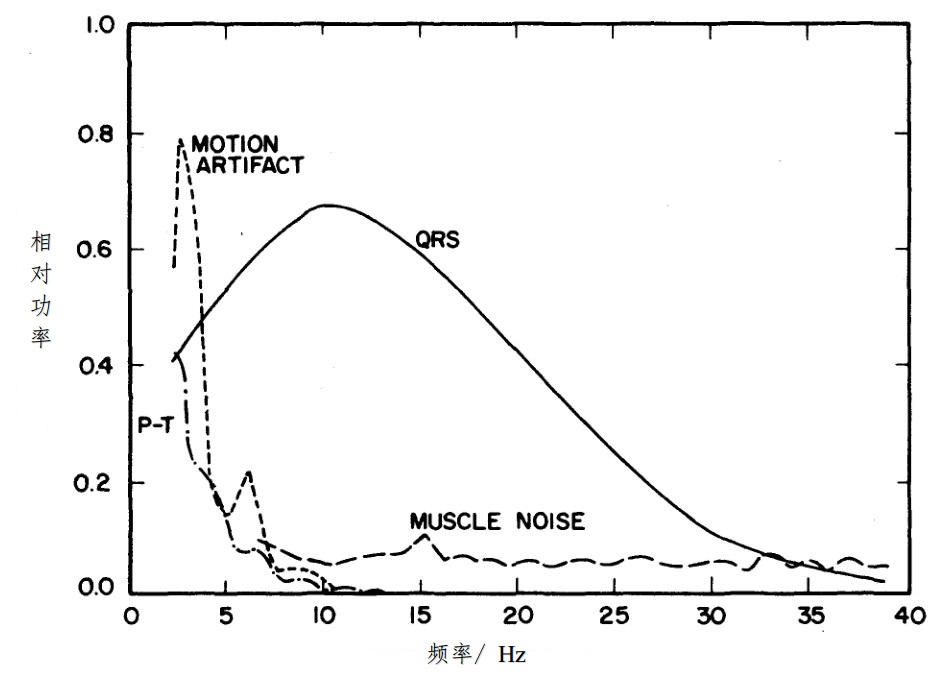
\includegraphics[width=.6\linewidth]{401}
    \caption{\label{fig:401}心电信号功率谱}
\end{figure}

由于数字滤波器的滤波精度高、算法设计灵活、可靠性高,各种基于数字滤波器的心电噪声抑制方法近年来不断涌现。 

(1) 平滑滤波器 

平滑滤波器是较早被人们采用的方法,该算法简单,处理速度快,滤波效果较好\cite{14}。其原理是基于多项式拟合方法设计的最佳简单形式的低通滤波器\cite{15}。
该方法对信号滤波时,实际上是拟合了信号中的低频成分,而将高频成分滤除。其基本的思路如下:对于信号$x(i),i=1,\dots,L$,构造一个$P$阶多项式
\begin{equation}
    \label{equ:401}
    f_i=a_0+a_1i+a_2i^{2}+\dots+a_pi^{p}=\sum_{k=0}^{p}a_ki^k,  p\le L-1
\end{equation}
以此来拟合信号。这个过程必然存在误差,设总拟合误差的平方和是 
\begin{equation}
    \label{equ:402}
    E=\sum_{i=1}^L[f_i-x(i)]^2=\sum_{i=1}^L[\sum_{k=0}^pa_ki^k-x(i)]^2
\end{equation}
为了使$E$最小,我们令$E$对个系数的导数为零,得
\begin{equation}
    \label{equ:403}
    \frac{\partial E}{\partial a_r}=\frac{\partial}{\partial a_r}[\sum_{i=1}^L(\sum_{k=0}^pa_ki^k-x(i))^2]=2\sum_{i=1}^L[\sum_{k=0}^pa_ki^k-x(i)]\cdot i^r = 0, r=1,2,\dots, p
\end{equation}
即
\begin{equation}
    \label{equ:404}
    \sum_{k=0}^pa_k\sum_{i=1}^Li^{k+r}=\sum_{i=1}^Lx(i)\cdot i^r
\end{equation}

在知道数据长度$L$,待拟合信号$x(i)$及拟合次数$p$后,就能够用\autoref{equ:404}求出系数$a_0,a_1,\dots,a_p$,因此多项式$f_i$也就可以确定\cite{16}。
当我们选择合适的数据长度$L$ 以及恰当的次数$p$ 时,得到的拟合多项式就是信号的趋势项,从信号中去除这部分就能够有效的抑
制基线漂移。

(2)小波阈值去噪

小波阈值去噪原理如下\cite{17,18}:

设含噪声一维信号模型为:
\begin{equation}
    \label{equ:405}
    x(i)=s(i) + \sigma \cdot e(i), i= 1, 2,\dots,L-1,L
\end{equation}
式中$s(i)$为有用信号,$e(i)$为噪声,$\sigma$为噪声方差。这里设噪声服从均值为零,方差为$\sigma$的高斯分布。

对\autoref{equ:405}两边同时进行小波变换,得到
\begin{equation}
    \label{equ:406}
    X=S+U, X=Wx, S=Ws,U=We
\end{equation}
噪声$e(i)$的协方差矩阵$Q$为:
\begin{equation}
    \label{equ:407}
    Q=E\{ee^T\}=\sigma^2I
\end{equation}
所以$P=E\{UU^T\}=E\{Wee^TW^T\}=WQW^T$,由于$W$是正交矩阵,则$P=Q=\sigma^2I$。即
经过小波变换之后,信号的能量主要集中在小波域内一些比较大的系数中,而相反的,
噪声的能量则被分散到整个小波域中。采用阈值法保留幅值比较大的信号小波系数,而
将噪声的系数置零或极大程度的抑制,再进行反变换重构信号,就能够达到去除噪声的
目的。

(3)中值滤波器

中值滤波是由排序统计理论衍生出的一种非线性的信号处理方法,是一种非线性滤
波器。基本思想是用信号中一个采样点邻域内各点的中值来代替该点的值,该方法可以
消除过大或过小的野点,最后得到信号的大体走势,即趋势项\cite{19}。

具体做法是:设置一个长度为$K$的矩形窗,从信号第$K$点开始,对于每一点$i$都用
以它为终点的长度为$K$的窗内数据的中值作为该点的值,最后得到的就是信号的趋势项,
即:
\begin{equation}
    \label{equ:408}
    Baseline(i)=median(x(i-K+1),x(i-K+2),\dots,x(i)),K\le i \le L
\end{equation}
其中,$L$为信号总长度,$median$函数的作用是求一段数据的中值。得到趋势项以后,将
其从原始信号中减去,就可以得到不含基线漂移的心电信号了。

\subsection{去噪方法的 Matlab 实现与对比分析}
针对第 3 章第 4 节所得的众多原始数据,我们选取了 113.dat 文件中提取的一通道数
据作为此次分析的样本数据。原始数据绘制的波形如\autoref{fig:402}所示。下面对几种常见算法
的去噪效果进行分析对比,为减少运算量,本文中截取了上述数据中的前 5000 个数据点
进行分析。

(1) 平滑滤波器

根据\autoref{equ:401},我们令$L=201,p=3$滤波后得到的趋势项以及去除基线漂移的结果如\autoref{fig:403}所示。平滑滤波器去除基线漂移的
效果很好,得到的趋势项相对平滑,对心电信号本身损害也比较少。但是由于需要对信号进行分段的多项式拟合,因而计算量偏大,计算时间较长。

\begin{figure}[htbp]
    \centering
    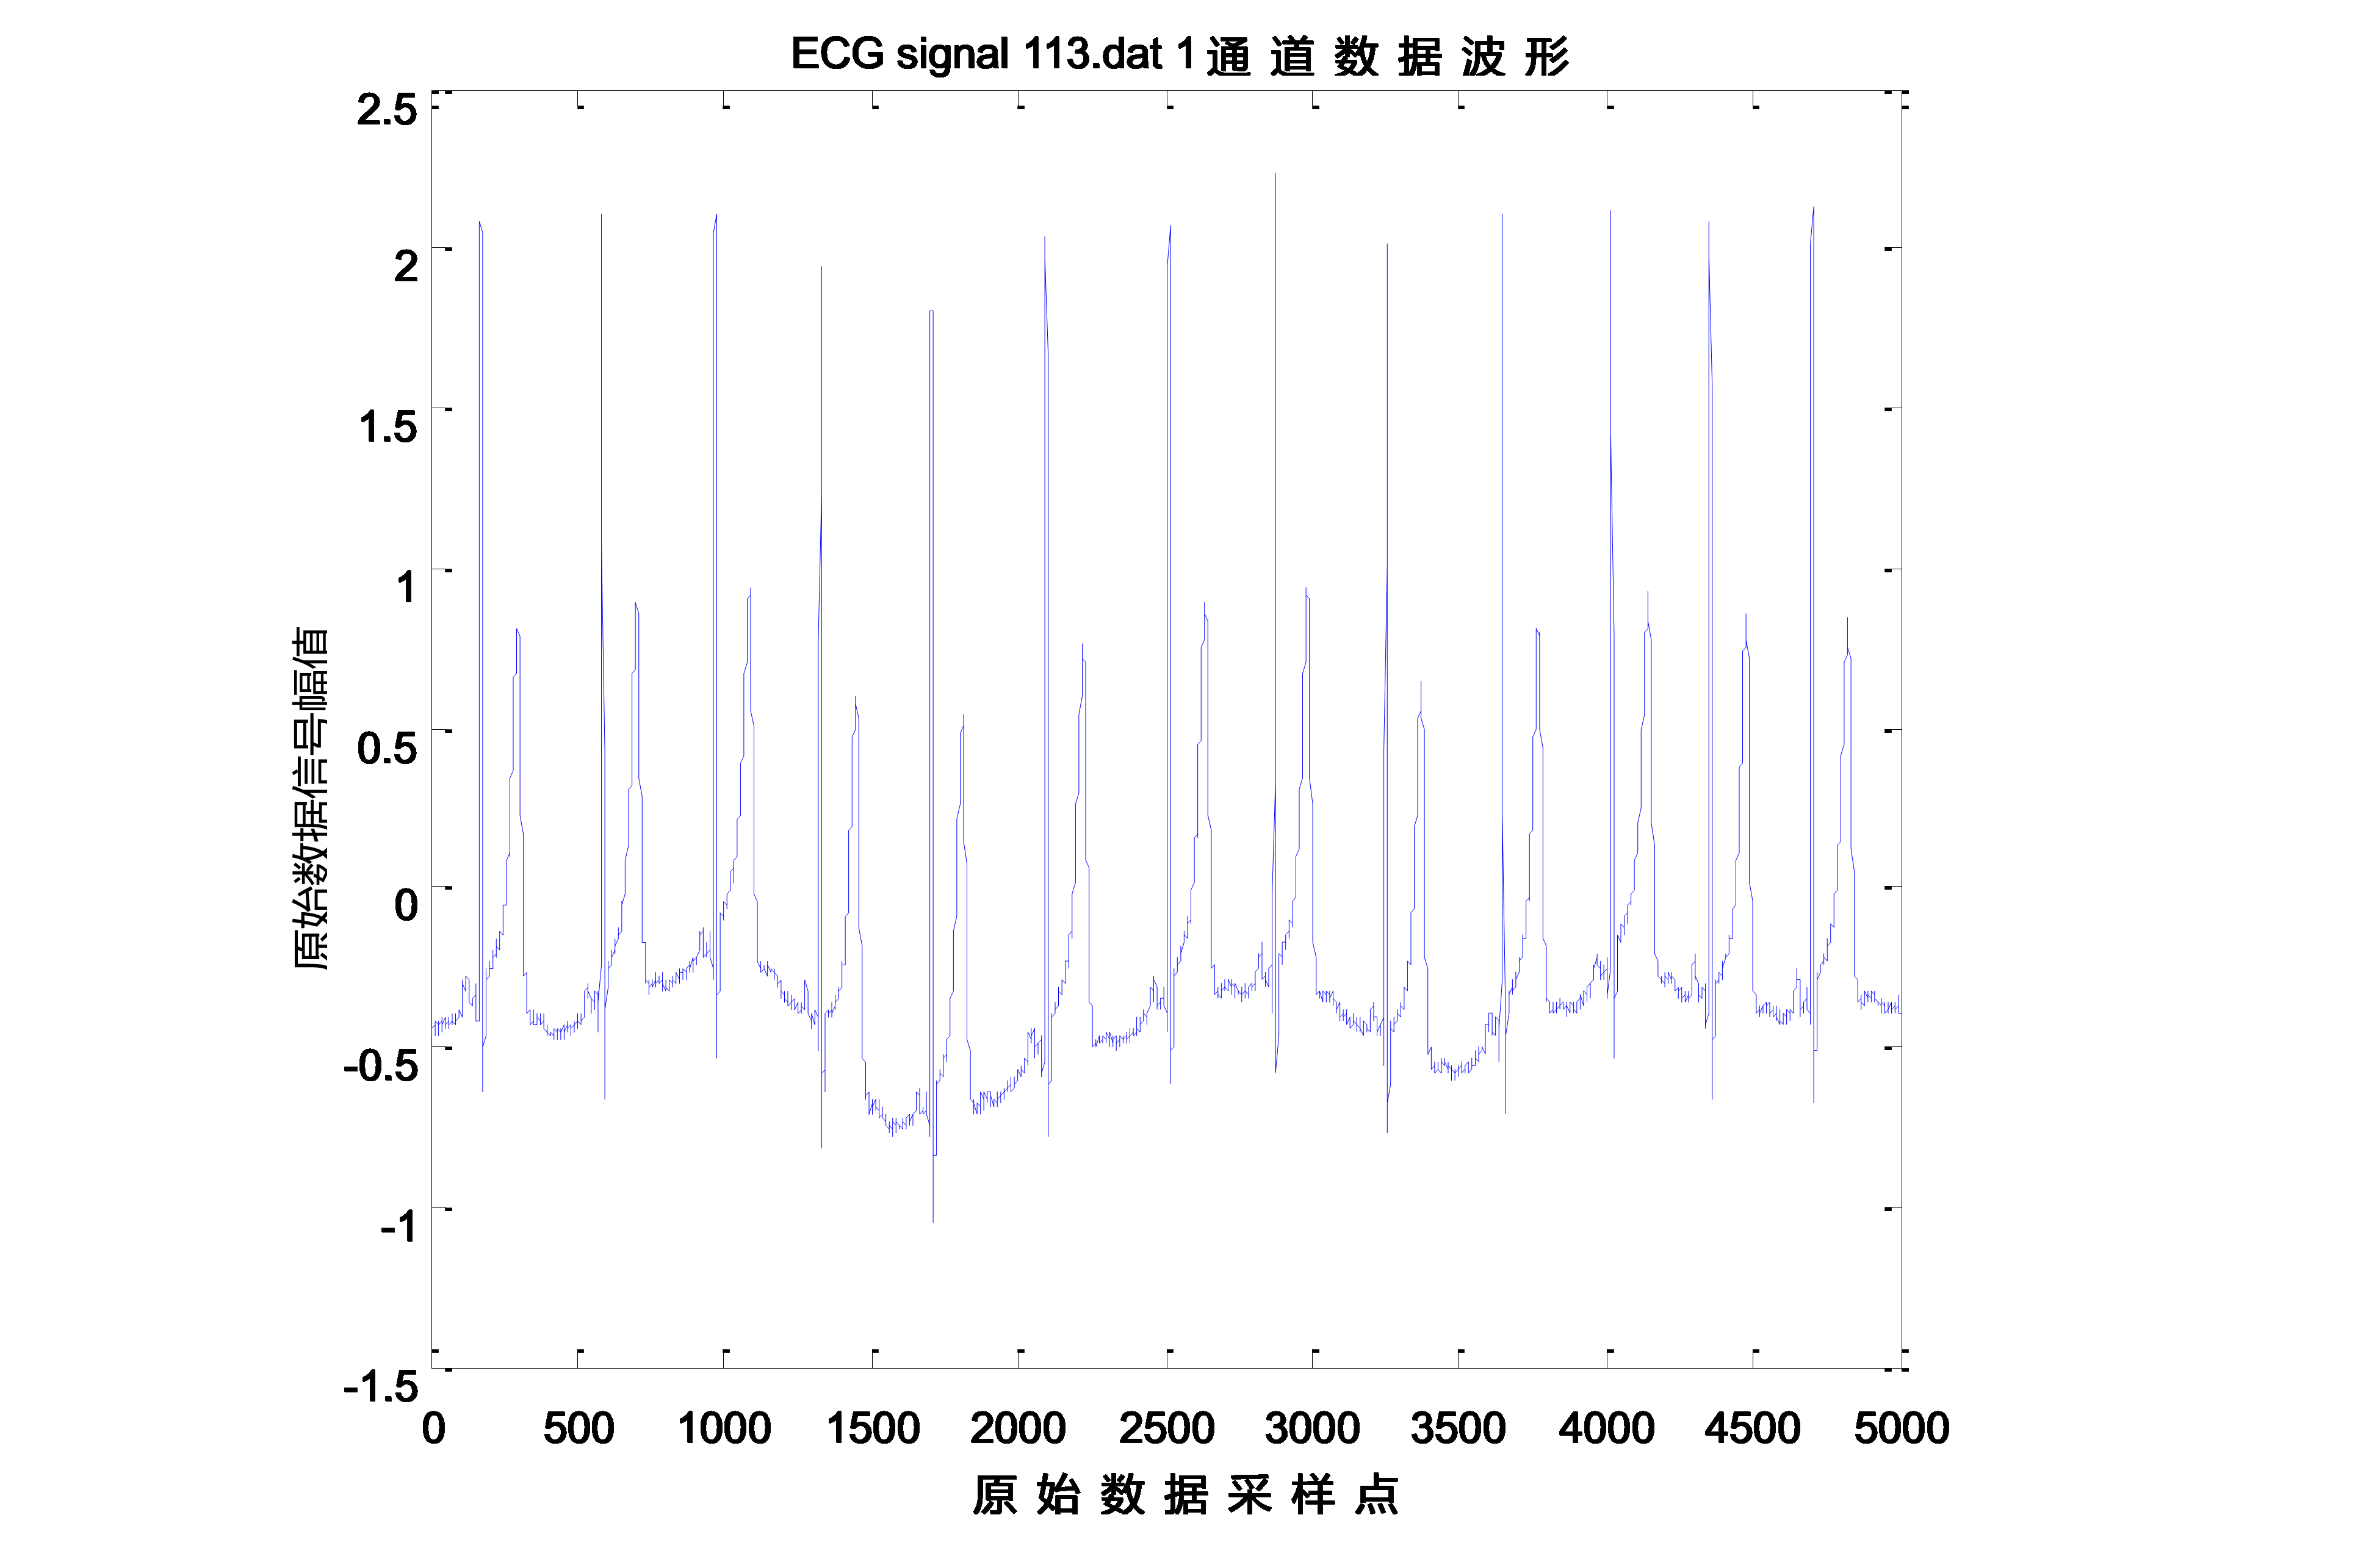
\includegraphics[width=.9\linewidth]{402}
    \caption{\label{fig:402}心电信号功率谱}
\end{figure}
\begin{figure}[htbp]
    \centering
    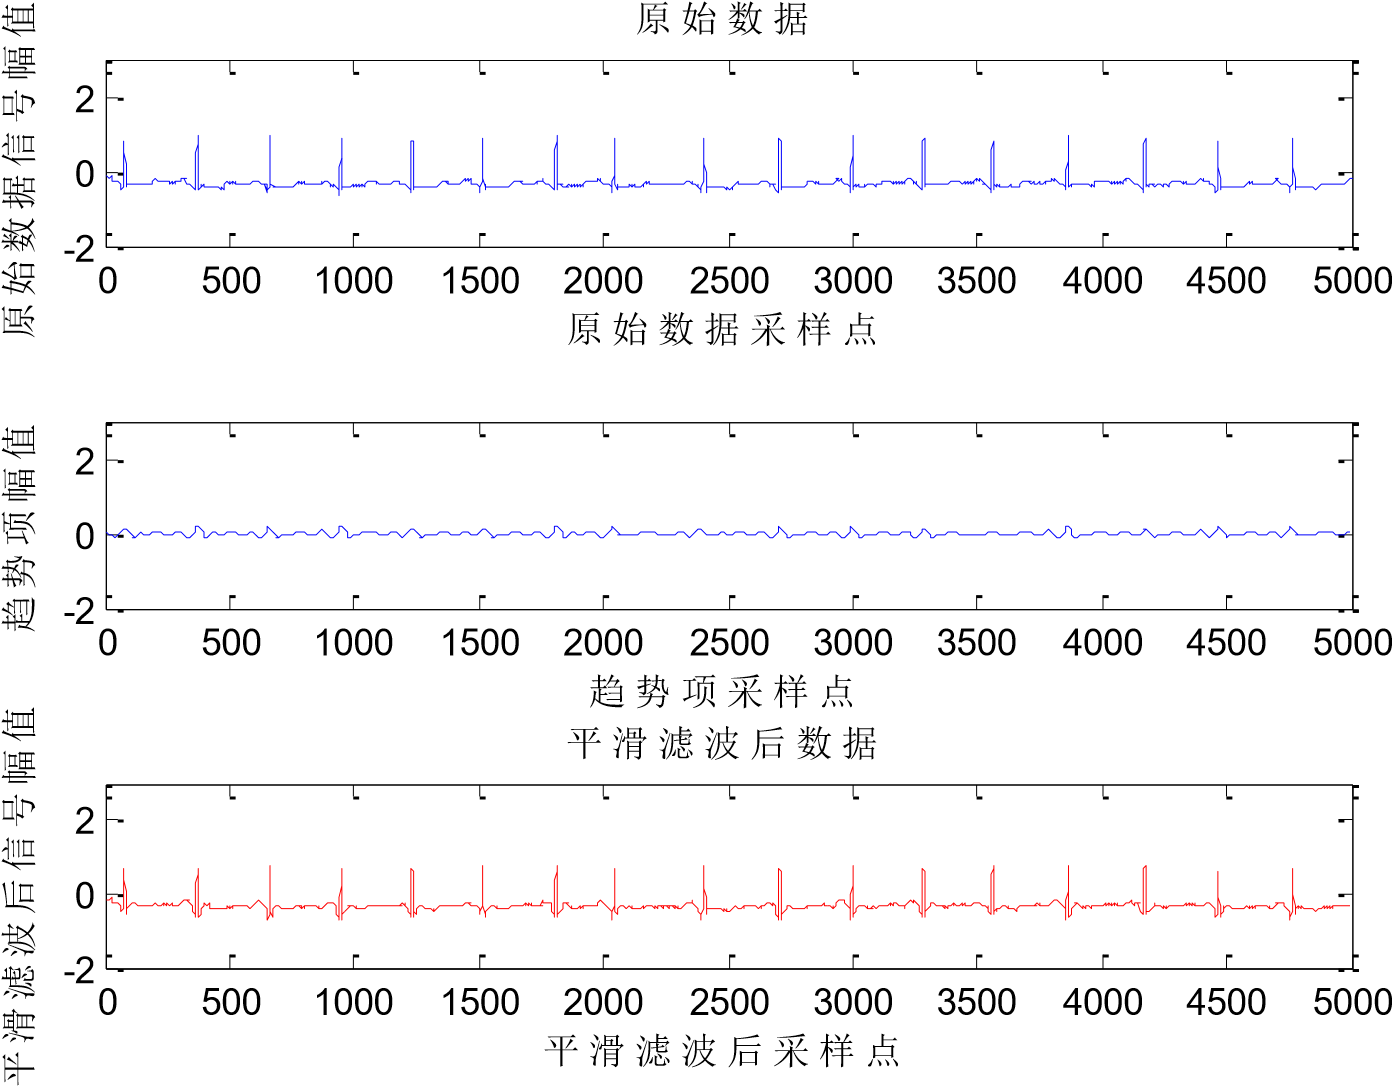
\includegraphics[width=.85\linewidth]{403}
    \caption{\label{fig:403}平滑滤波去除基线漂移效果图}
\end{figure}

(2)	小波阈值去噪 

我们采用软阈值去小波滤波器去噪,从其效果\autoref{fig:404}可以看到,该方法可以有效的
去除高频噪声,同时波形没有发生畸变,幅度也没有明显衰减。 
\begin{figure}[htbp]
    \centering
    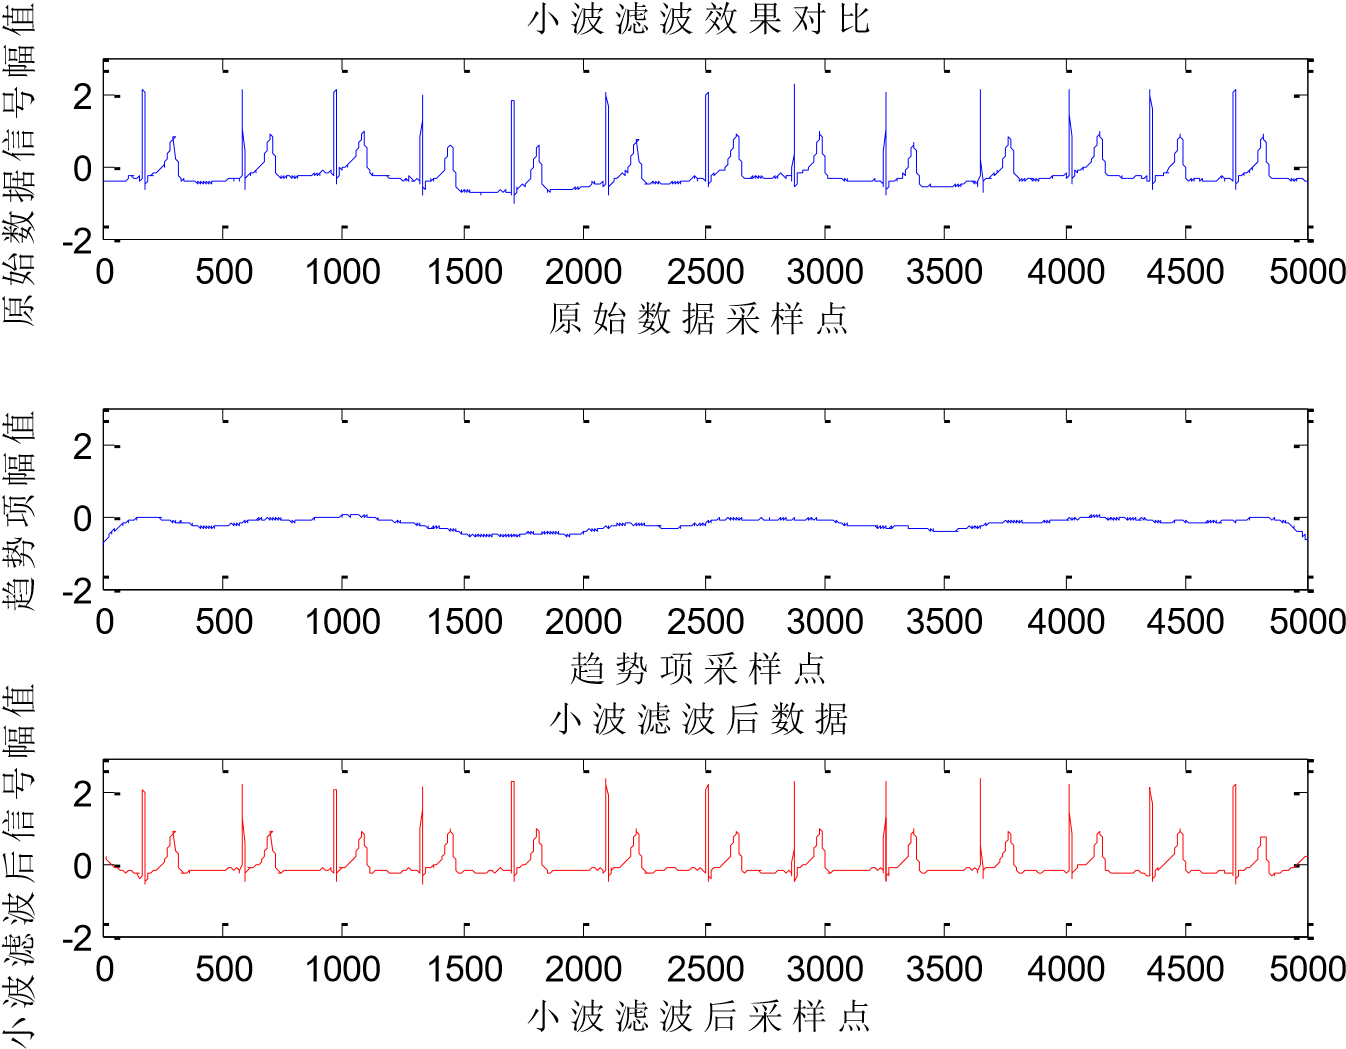
\includegraphics[width=.85\linewidth]{404}
    \caption{\label{fig:404}小波阈值去噪效果图}
\end{figure}

(3)	中值滤波器 

我们测试多个窗长参数$K$,最终选定的$K = 100$。滤波效果如\autoref{fig:405}所示,该方法去基线漂移效果较好,值得注意的是由于有窗长 $K$的要求,
滤波后的信号必然有 $K$ 点保持原始信号,其始端或者是尾部(由滤波从哪里开始决定)会有异常,按照我们的做法,数据初始有 100 点不能去除基线,
由于原始信号基线幅度很大,导致这 100 点数据异常较为明显。 
\begin{figure}[htbp]
    \centering
    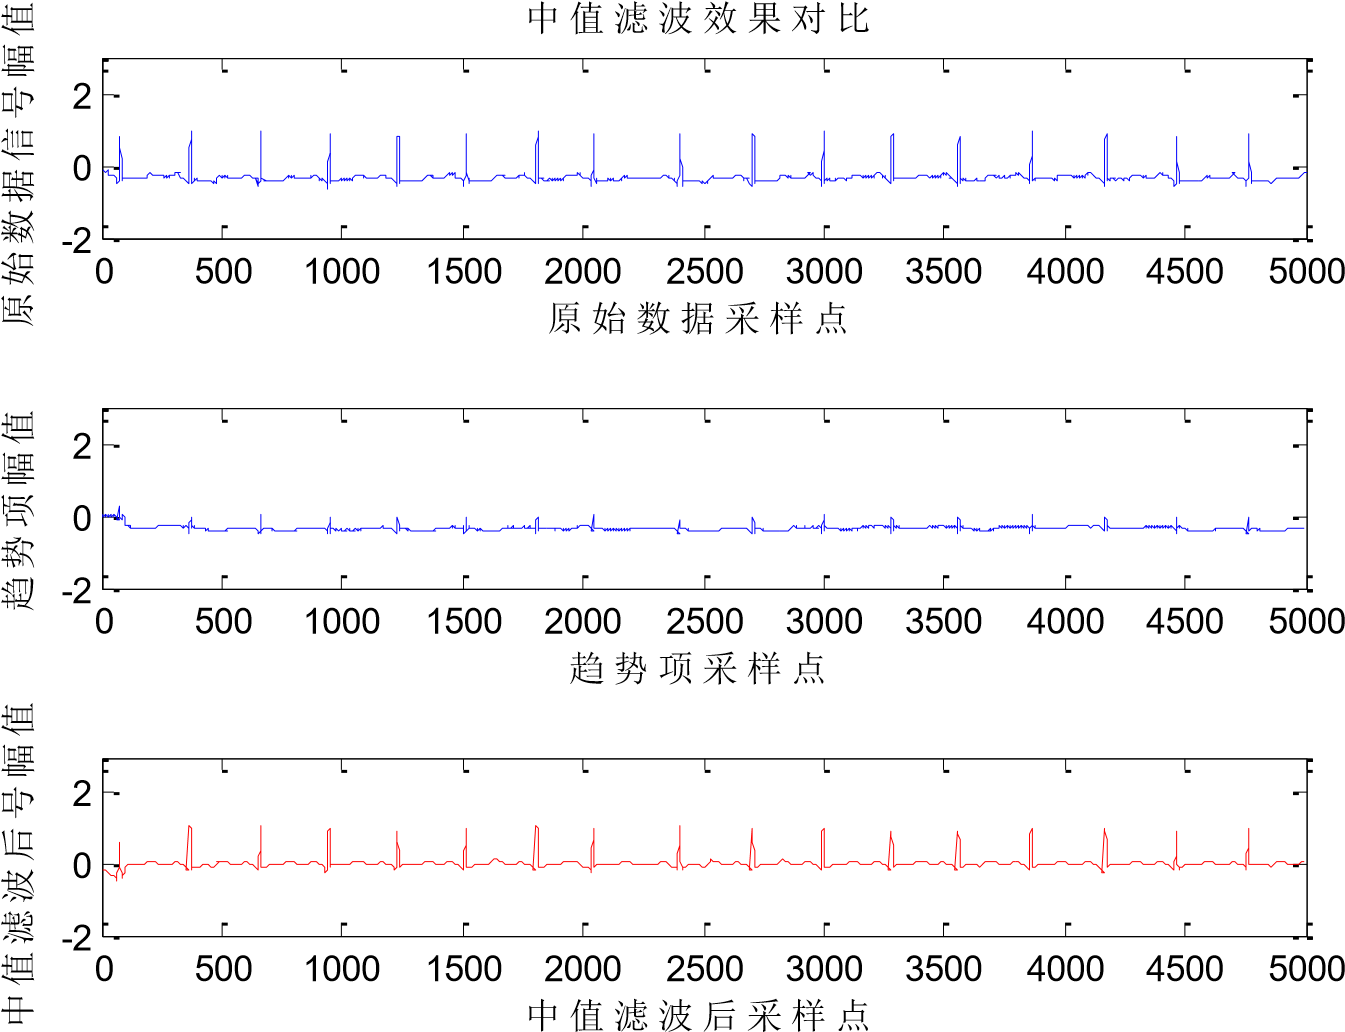
\includegraphics[width=.85\linewidth]{405}
    \caption{\label{fig:405}中值滤波去除基线漂移效果图}
\end{figure}

(4)	几种滤波器滤波效果的对比 

对以上滤波方法的滤波效果量化对比,主要考察的因素有: 

\ding{172}直观的滤波效果与波形幅值衰减与否:主观观察进行评价。 

\ding{173}时间复杂度:通过 Matlab 的自带函数$tic$ 与 $toc$ 直接计算。其数值越小,算法越优秀。 

\ding{174}信噪比:计算公式: 
\begin{equation}
    \label{equ:409}
    SNR=10 \times log_{10}\sum_{i=1}^L\frac{y_i^2}{(x_i-y_i)^2}
\end{equation}
其中 $y$ 与 $x$ 分别是原始数据与滤波后的数据,$SNR$ 数值越大,算法越优秀。 

\ding{175}均方误差:计算公式: 
\begin{equation}
    \label{equ:410}
    MSE=\frac{1}{L}\sum_{i=1}^L(y_i-x_i)^2
\end{equation}
其中 $y$ 与 $x$ 分别是原始数据与滤波后的数据,$MSE$ 其数值越小,算法越优秀。最后的对比结果,如\autoref{tab:401}所示。
从中可以看到,平滑滤波的对原始信号幅值的衰减最为严重,且算法运行时间最长,小波变换的滤波性能最为优秀,平滑滤波则在算法的时间复杂度上表现最为优秀。 

\begin{longtblr}
    [
        theme          = {dut},
        caption        = {几种滤波方法效果对比},
        label          = {tab:401},
    ]
    {
        colspec        = {X[2,c,m]X[1,c,m]X[1,c,m]X[1,c,m]},
        hline{1,Z}     = {\thickline},
        hline{2}       = {\thinline},
        rowhead        = 1,
        row{odd}       = {bg=\oddcolor}, 
        row{even}      = {bg=\evencolor},
        row{1}         = {font=\headfont,bg=\headcolor},
        row{2-Z}       = {font=\nonheadfont},
    }
    效果考察项 & 平滑滤波 & 	小波变换滤波 &	中值滤波 \\
    直观的滤波效果 &	滤波效果一般 & 滤波效果较好 & 滤波效果较好 \\
    波形幅值衰减是否明显 &	衰减明显 &	无明显衰减 	& 无明显衰减 \\
    信噪比(db) &	1.5903& 	5.1459 &	1.2983 \\
    均方误差 & 0.1581 &	0.0697 &	0.1691 \\
    信噪比/均方误差 &	10.0583 &	73.8020 &	7.6774  \\
    处理时间(s) &	0.9011 &	0.4300 	&0.0619  \\
\end{longtblr}

\subsection{中值滤波算法在智能手机环境下的改进与实现 }
在综合考虑滤波算法的性能之后,本文设计最终移植了中值滤波算法到 Android 系统下,进行心电数据的预处理过程。由于上文提及的中值滤波算法在 Matlab 上实现时,
有可直接使用的求取一定窗口数据的中值的函数存在,而在 Android 下需重新在底层构建中值滤波的算法。一般而言,传统的中值滤波算法是基于排序的,
大量的无用的排序与交换工作被重复进行,导致中值滤波算法的效率与实际可行性将大大降低。在前人研究的基础上\cite{20},本文对中值滤波算法进行了优化,
充分利用了窗口移动时,移入值与移出值对新旧中值可能的影响,在确定了数据变化的位置关系后,完成相应的数据插入与删除,大大减少了数据的排序量,
从而实现中值的快速计算。经在 Matlab 仿真,改进后的算法与使用 Matlab 自带函数对同一段数据进行分析处理的结果完全相同,
在执行的效率上甚至略有提高,时间对比如\autoref{tab:402}所示。由于算法的实现不基于任何集成的算法或函数,因此具有良好的移植性。 
\begin{longtblr}
    [
        theme          = {dut},
        caption        = {优化前后的中值滤波算法效率对比},
        label          = {tab:402},
    ]
    {
        colspec        = {X[2,c,m]X[1,c,m]},
        hline{1,Z}     = {\thickline},
        hline{2}       = {\thinline},
        rowhead        = 1,
        row{odd}       = {bg=\oddcolor}, 
        row{even}      = {bg=\evencolor},
        row{1}         = {font=\headfont,bg=\headcolor},
        row{2-Z}       = {font=\nonheadfont},
    }
    算法 &	处理时间(s) \\
    Matlab集成中值滤波算法 & 	0.0619 \\
    优化后的中值滤波算法 	& 0.0607 \\
\end{longtblr}
现将该算法原理介绍如下: 

(1)	第一次求出窗口数的中值。设中值滤波的窗口数为$2N+1$,算法的第一遍求前 $2N+1$ 个数的中值需进行一次简单的冒泡排序即可。 

(2)	利用数据的相关性计算中值。我们发现窗口在移动时,中间 $2N$ 个数是不变的,因此影响新中值的数值不外乎三个数据,新移入窗口的数据(移入值),
移除窗口的旧值(移出值)以及上一次窗口的中值(旧中值)。我们将移入值、移出值分别与旧中值比较,若两者都大于等于或者小于等于旧中值,则用移出值替
换移入值的位置即可,新中值在数值上与旧中值相同;若旧中值在两者数值之间,则相应在大于旧中值或小于旧中值的部分求取最小值或最大值,该值即为新中值。

(3)	算法的评价。本文算法主要工作是进行两次比值后决定在 $N$ 个数中寻找到最大(小)值,这仅需一次遍历即可实现。若处理数据总长度为 $M$,
则该算法的实现复杂度约为$O(M\cdot N)$,相较排序求中值算法的$O(M\cdot N^2)$的时间复杂度,大大提高了执行效率。 

\section{心电信号的特征提取算法}
临床上,医生对于某种心脏疾病进行诊断时,最重要的依据就是病人心电图的异常情况,而判断是否异常的准则就是心电波形各个波段的指标。
心电信号特征点检测的目的就是在预处理的基础上,使用各种有效的信号处理方法,准确的检出波形,并精确定位各个特征点,将复杂的心电信号
转化为较为容易分析的形式,以便于后期分析波形参数以及形态的特征,为心脏疾病自动诊断提供信息。 

\subsection{R波检测}
R 波是心电图中最具代表性的波形,其幅值远高于其他段的波形,因此,在实际的分析过程中,R 波最容易被检测,且检测方法较为成熟,
常见的检测算法有固定阈值法、可变阈值法、小波变换法等算法。通常人们把 R 波作为一个心跳周期的标志,RR 间期则是用来计算心率大小的标准数据。
在本文中,选取了固定阈值法来检测 R 波。 

算法原理如下: 

(1) 对原始信号进行处理,将原始数据进行斜率计算保存成新的处理数据, 

(2)	将上步所得的数据,分成若干组遍历出各组的最大值,求出各组最大值的平均值,作为此次 R 波检测过程的阈值。

(3)	遍历第一步所得数据,若某点的数值大于阈值,则该点可能为一个 R 波位置,计算此点与上一个 R 波距离,若两者距离超出不应期则判断该点为一个新 R 峰。 

这种算法对于 R 峰漏检的预防体现在设立了一个标识符,初始化为 0,若出现已检测出 R 峰,但下一超过阈值与 R 峰的距离超出了不应期的距离,则说明出现了漏检的情况,
处理方法是将阈值乘以一定的系数(一般为小于 1 的正值,可人工设定为 0.6-0.8)缩小后重新对上一 R 峰之后的数据段进行检测。 

\subsection{QRS波群始末点的检测}
在上一小节检测出 R 峰的基础上,对 QRS 波群的始末点的检测可按如下局域变换算法进行\cite{21,22}: 

局域变换法的基本思想,是用心电信号减去一段斜率不变的直线,以将心电信号中斜率的变化用$abs(D)$表示,然后选取绝对值最大的点为所检测的点即为斜率变化最大的点。
QRS 波起始点的检测是在 R 波及 R 波的起始点和结束点正确检测的基础上进行检测,那么这条直线的建立也是以确定了 R 波位置为前提的。
$y(i)$直线公式如\autoref{equ:411}所示,斜率变化由\autoref{equ:411}所示: 
\begin{equation}
    \label{equ:411}
    y(i)=x(i_1)+\frac{x(i_2)-x(i_1)}{i_2-i_1}(i-i_1)
\end{equation}
\begin{equation}
    \label{equ:412}
    D(i)=x(i)-y(i)
\end{equation}
式中$i_1$和$i_2$为心电信号$x(i)$上两点。 
\begin{figure}[htbp]
    \centering
    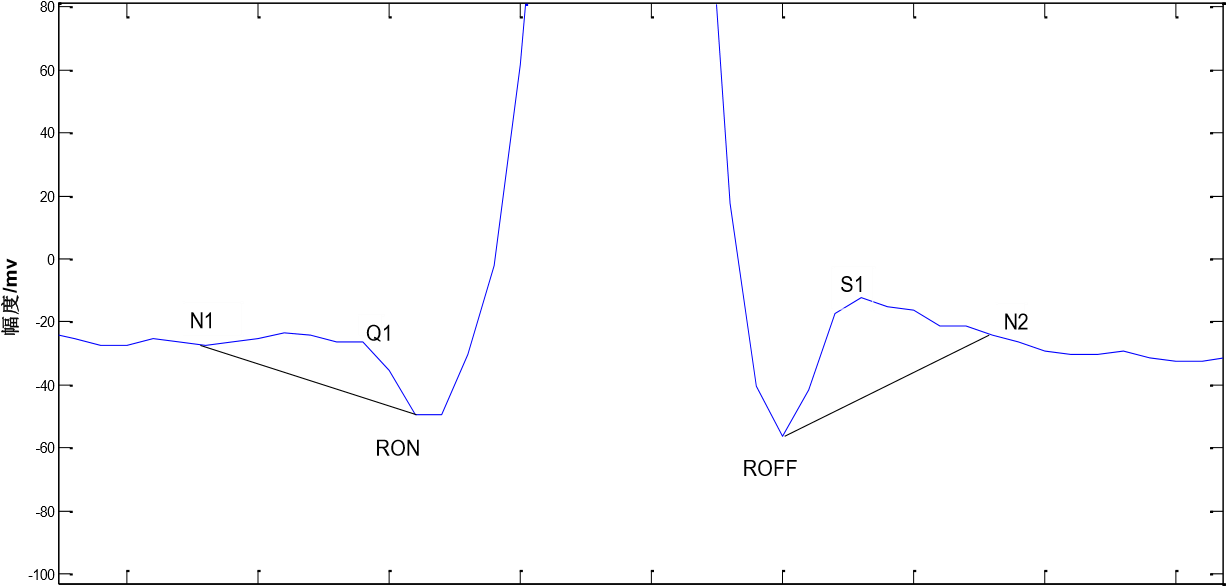
\includegraphics[width=.85\linewidth]{406}
    \caption{\label{fig:406}QS点检测示意图}
\end{figure}

\autoref{fig:407}为心电信号 QS 点检测示意图,在 R 波起始点$R_{ON}$和 R 波结束点$R_{OFF}$ 定位之后,通过$N1$点和$R_{ON}$构建一条直线 
$y_Q(i)$ 并计算$D_Q(i)$,判断 $Q$、$S$ 点存在的具体步骤如下: 

(1)	寻找$D_Q(i)$中绝对值最大值点$Q_1$; 

(2)	若$x(Q_1)>y_Q(Q_1)$则认为存在 Q 波,点$Q_1$即为 $Q $点并作为$QRS_{ON}$点,否则认为不存在 Q 波,$R_{ON}$作为$QRS_{ON}$点; 

(3)	S 点的检测采用同样的方法; 

\begin{figure}[htbp]
    \centering
    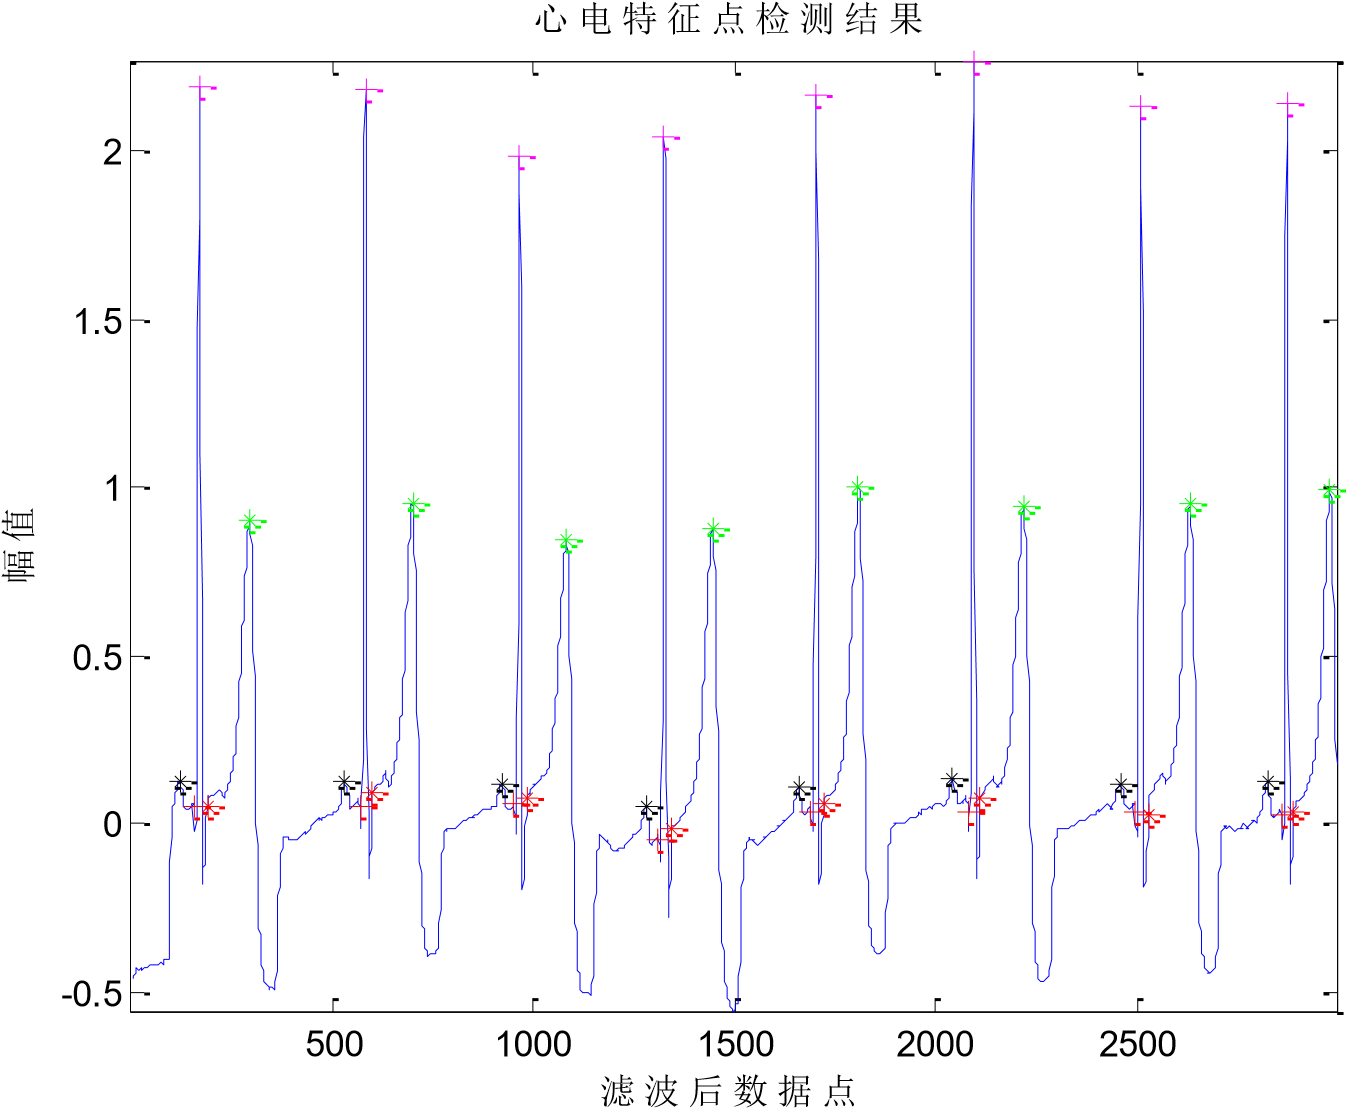
\includegraphics[width=.85\linewidth]{407}
    \caption{\label{fig:407}Matlab上的特征点检测效果}
\end{figure} 

\subsection{P波与T波波峰检测}
在前面两小节检测的基础上,P 峰与 T 峰的检测工作相对来说简单。在心电波形上可知,P 峰 T 峰与 R 峰有着类似的性质。因此检测算法也类似。
仅检测的始末点略有区别。P 峰的检测始点为当前 R 峰根据 PR 间期的确定点开始,到 QRS 波群的起点终止。 T 峰检测的起点为 QRS 波群的终点,
到根据 RT 间期关系确定的点终止。分别在这两段数据的斜率进行遍历,该段数据点斜率的最大值即为我们要求的 P(T)峰。由于在 R 峰检测过程中已经
考虑了漏检的状况,对相应 P 峰与 T 峰的检测则可以省略这个过程。 

\subsection{心电特征检测效果}
在前 3 节的基础上,我们将相应的算法改写后成功分别在 Matlab 与 Android 系统的上实际运行了。Matlab 的运行效果如\autoref{fig:407}所示,
在 Android 系统运行效果如\autoref{fig:408}所示。 

\begin{figure}[htbp]
    \centering
    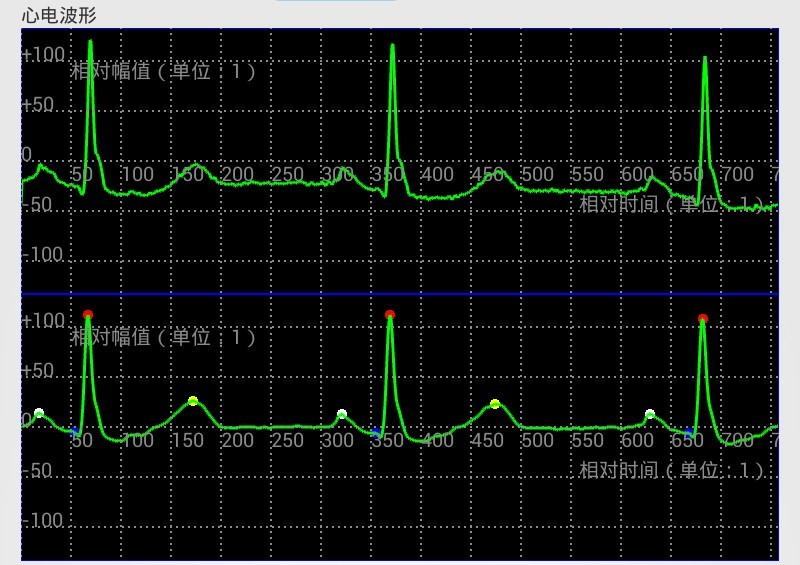
\includegraphics[width=.85\linewidth]{408}
    \caption{\label{fig:408}智能手机上的特征点检测效果 }
\end{figure}

为进行直观对比,我们将 Android 下与 Matlab 下特征点检测值对比如表 4.2 所示。值得注意的是,Android 下数组的起始坐标为 0,而 Matlab 下的起始坐标为 1。可以看
到,两者的运行效果误差很小,趋近一致。 

\begin{longtblr}
    [
        theme          = {dut},
        caption        = {Anroid 与 Matlab 心电特征检测结果对比},
        label          = {tab:403},
    ]
    {
        colspec        = {X[2,c,m]X[2,c,m]X[1,c,m]X[1,c,m]X[1,c,m]X[1,c,m]X[1,c,m]X[1,c,m]X[1,c,m]X[1,c,m]},
        hline{1,Z}     = {\thickline},
        hline{2}       = {\thinline},
        rowhead        = 1,
        row{2-3,6-7,10-11} = {bg=\oddcolor}, 
        row{4-5,8-9}      = {bg=\evencolor},
        row{1}         = {font=\headfont,bg=\headcolor},
        row{2-Z}       = {font=\nonheadfont},
        cell{2,4,6,8,10}{1}  = {r=2,c=1}{c,m},
    }
    心电特征 & 算法语言 & 1 & 2 & 3 & 4 & 5 & 6 & 7 & 8 \\
    P 峰 &	Java & 118 & 529 & 919 & 1276 & 1656 & 2040 & 2458 & 2821 \\
        &Matlab &	119 & 530 & 920 & 1277 & 1657 & 2041 & 2459 & 2822 \\
    QRS 起点&  	Java & 154 & 566 & 950 & 1310 &1688 & 2077 & 2494 & 2856\\
        &   Matlab & 154 & 567 & 951 & 1311 & 1689 & 2078 & 2495& 2857\\ 
    R 峰 & 	Java & 168	& 580 & 964 & 1324 & 1702 & 2091 & 2508 & 2870 \\ 
        & Matlab & 169 & 581 & 965 & 1325 & 1703 & 2092 & 2509 & 2871 \\
    QRS 终点 & Java & 187 & 599 & 982 & 1343 & 1720 & 2110 & 2527 & 2888\\
        & Matlab & 188 & 600 & 983 & 1344 & 1721 & 2111 & 2528 & 2889 \\
    T 峰 &	Java & 293 & 696 & 1080 & 1443 & 1806 & 2216 & 2630 & 2978 \\
        & Matlab & 294 & 698 & 1081 & 1444 & 1807 & 2217 & 2631 & 2979 \\
\end{longtblr}

\section{本章小结}
本章在前几章的基础上,实现了对实际获取的人体心电信号数据分析处理的过程,着重研究了去噪过程与信号特征提取过程的算法实现及评价上。在去噪算法模块,
着重考虑了噪声的干扰及基线漂移在心电信号检测过程中的影响,对比了平滑滤波、小波滤波及中值滤波算法的去噪效果,并在前人的基础实现了中值滤波算法的优化并在
Android 上成功移植。在特征提取方面,使用了斜率阈值的方法首先提取出了 R 波的位置,并以此为基础,依次确定了其他特征值的位置。
以上算法均在 Matlab 上进行了仿真与处理,并在 Android 上取得了基本一致的检测效果。

